\documentclass[11pt,a4paper]{article}
\usepackage[T1]{fontenc}
\usepackage{lmodern}
\usepackage[margin=23mm]{geometry}
\usepackage{amsmath,amssymb,amsthm,booktabs,graphicx,microtype,xcolor}
\usepackage[colorlinks=true,linkcolor=teal,citecolor=teal,urlcolor=teal]{hyperref}
\newtheorem{theorem}{Theorem}
\newtheorem{lemma}[theorem]{Lemma}
\newcommand{\diag}{\operatorname{diag}}
\newcommand{\doi}[1]{\href{https://doi.org/#1}{doi: #1}}
\hypersetup{pdftitle={When can weak site potentials restore a molecular transmission zero?},pdfkeywords={molecular quantum interference, Hückel model, radialenes, Green function}}
\title{When can weak site potentials restore a molecular transmission zero?}
\author{Research note}
\date{}
\begin{document}
\maketitle
\begin{abstract}
At a fixed off-resonant energy, a coherent molecular junction may have zero transmission between two contacts. If the signs of local site-energy shifts are prescribed, can the zero recur with every shift nonzero and arbitrarily small? We give a necessary and sufficient criterion using the signs of chordless paths in the unperturbed Green-function graph. The proof identifies the inclusion-minimal monomials of the transmission cofactor. For a nearest-neighbour $[n]$radialene model with nonadjacent exocyclic contacts, positive shifts can compensate on odd rings, whereas every sufficiently weak positive choice opens the zero on even rings. When the two ring arcs have $p$ and $q$ internal sites, the compensation curve scales as $x\sim C y^{q/p}$. This exponent survives arbitrary positive changes of the ring and exocyclic hopping magnitudes. For $[5]$radialene with unit hopping the curve is $x=y^2/(1-y^2)$.
\end{abstract}

\section{A zero missed by proportional gate sweeps}
Consider the ten carbon $\pi$ orbitals of $[5]$radialene. Take one orbital per carbon, zero parent site energies, nearest-neighbour hopping $-1$, and tunnelling energy $E=0$. Put the contacts on exocyclic carbons whose neighbouring ring atoms are two bonds apart. Of the three remaining exocyclic sites, shift the one on the shorter arc by $x$ and both on the longer arc by $y$ (Fig.~\ref{fig:curves}). The isolated-core Green function between the contacts is exactly
\begin{equation}
 F(x,y)=x-\frac{y^2}{1-y^2}. \label{eq:five}
\end{equation}
At $y=1/10$, choosing $x=1/99$ restores zero transmission. Choosing $x=y=1/10$ gives $F=89/990$. Every fixed ray $x=c y$ with $c>0$ has $F>0$ for all sufficiently small $y>0$, even though exact zeros accumulate at the origin within the positive quadrant. Section~\ref{sec:rad} derives the formula from the Hamiltonian. The synthesis of the parent hydrocarbon is documented in Ref.~\cite{mackay}. Its transport response here is a model prediction.

\begin{figure}[!ht]
\centering
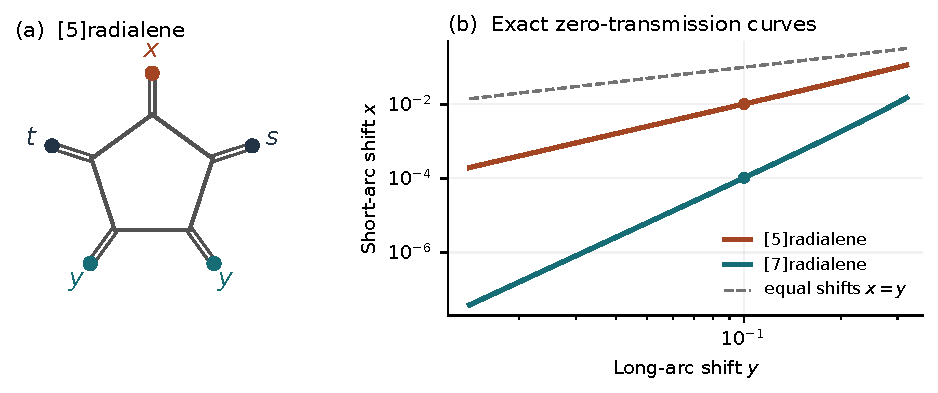
\includegraphics[width=.84\linewidth]{radialene_figure.pdf}
\caption{(a) The two contacts and the three shifted exocyclic sites. (b) The exact positive compensation curves for the five- and seven-membered ring models with one short-arc gate. Dots mark $y=1/10$. Both axes use the hopping magnitude as the energy unit and logarithmic scales. The dashed line represents an equal-amplitude sweep.}
\label{fig:curves}
\end{figure}

The unperturbed inverse graph, its response to local impurities, and molecular logic-gate examples have been studied by Ni\c{t}\u{a} and co-workers~\cite{nita22,nita23}. Their shortest-path rule gives the lowest possible perturbation order~\cite[Secs.~3--4]{nita25}. Birkinshaw and co-workers identify the unperturbed radialene inverse graph through the corona construction~\cite[Sec.~5.1]{birkinshaw}. First-principles calculations have also considered a radialene with four leads~\cite{saha}. The question addressed here concerns simultaneous strictly nonzero shifts with prescribed signs whose magnitudes can approach zero at different rates. In Eq.~\eqref{eq:five}, the shortest path gives the linear term but a longer path sets the compensation scale.

\section{A signed-path criterion}
Let $H$ be a finite real symmetric single-particle Hamiltonian, $M=EI-H$ invertible at real $E$, and $g=M^{-1}$. Assume $s\ne t$ and $g_{st}=0$. Choose a set $S$ of sites other than $s,t$, prescribe $\sigma_i\in\{-1,1\}$ on $S$, and write $D_{ii}=\sigma_i x_i$ there. All other matrix entries of $D$ are zero. Define
\[
 F(x)=[(M-D)^{-1}]_{st}.
\]
The graph on $S\cup\{s,t\}$ has edge $ij$ whenever $i\ne j$ and $g_{ij}\ne0$. Its edges may join atoms that share no chemical bond. A chordless $s$--$t$ path is a simple path on whose vertices the graph induces exactly that path. Let $I(P)$ be its internal sites and set
\[
 a(P)=\prod_{ij\in E(P)} g_{ij}\ \prod_{i\in I(P)}\sigma_i .
\]
Changing orbital phases by signs multiplies every $a(P)$ by the same contact sign, preserving their agreement or disagreement.

\begin{theorem}\label{thm:sign}
If the graph has no $s$--$t$ path, then $F$ vanishes identically wherever the inverse exists. If there is at least one path and the $a(P)$ of all chordless paths have the same sign, then $F$ has that strict sign throughout $(0,h)^S$ for some $h>0$. If two chordless paths have opposite signs, then every sufficiently small open cube $(0,h)^S$ contains positive and negative values of $F$, as well as an exact zero.
\end{theorem}

\begin{lemma}\label{lem:monomials}
Define $Q(x)=\det(M-D)/\det M$ and $N(x)=Q(x)F(x)$ by cofactor continuation. The inclusion-minimal supports of nonzero monomials in $N$ are exactly the $I(P)$ of chordless $s$--$t$ paths. The coefficient of $x_{I(P)}=\prod_{i\in I(P)}x_i$ is $a(P)$.
\end{lemma}
\begin{proof}
Cramer's rule makes $N$ a normalized cofactor of $M-D$. It is affine in each variable separately, and $Q(0)=1$. Set all shifts outside an arbitrary $A\subseteq S$ to zero. Near zero the Neumann series for $F$ is
\[
 g_{st}+\sum_{k\ge1}\ \sum_{i_1,\ldots,i_k\in A}
       g_{s i_1}D_{i_1 i_1}\left(\prod_{j=2}^k g_{i_{j-1} i_j}D_{i_j i_j}\right)g_{i_k t}.
\]
A nonzero term gives a walk through $A$ (diagonal steps are permitted). Deleting repetitions gives a path. With no such path the restricted $N$ vanishes on a neighbourhood, hence identically as a polynomial. If $A=I(P)$ for a chordless path, deleting any site breaks the connection. The unique shortest walk is the path itself, giving lowest term $a(P)x_A$. Multiplication by $Q$ preserves this term. Conversely any minimal nonzero support $A$ must connect the contacts, so it contains the internal sites of a shortest path in the graph restricted to $A\cup\{s,t\}$. This path is chordless and its support already has a nonzero coefficient. Minimality forces equality.
\end{proof}

\begin{proof}[Proof of Theorem~\ref{thm:sign}]
The empty-path case follows from the lemma. Otherwise assign each nonminimal monomial of $N$ to any minimal monomial dividing it. Because $N$ is multiaffine this gives the finite expansion
\[
 N(x)=\sum_{P\ \mathrm{chordless}} x_{I(P)}\big(a(P)+R_P(x)\big),\qquad R_P(0)=0.
\]
There is one $h>0$ small enough that $Q>0$ and every bracket keeps its constant sign on $[0,h]^S$. When these signs agree, each term has that strict sign in the interior, regardless of the relative sizes of the $x_i$. For mixed signs, take the corner with $x_i=h$ on one chordless path's internal sites and zero elsewhere. Only its minimal monomial survives there. The corner for the opposing path has the other sign. Continuity moves both signs into the open cube, and the segment between the two interior points contains a zero.
\end{proof}

\paragraph{A finite-amplitude check.}
On any closed box with nonempty interior where $Q>0$, $N$ at an interior point is an average of its corner values with strictly positive multilinear interpolation weights. Unless $N$ is identically zero, it has an interior zero exactly when two corners have opposite signs. This is the multiaffine vertex principle (compare Ref.~\cite{vertex}). The path criterion gives the local possibilities directly from $g$. Related path decompositions of inverse entries appear in the Gaussian graphical-model setting~\cite{jones}.

\paragraph{Contacts and transmission.}
Write $f=(M-D)^{-1}$. With one local contact at each of $s,t$ and diagonal retarded self-energies $\Sigma_s,\Sigma_t$, inversion of the two-site Dyson equation gives
\[
 {\cal G}_{st}=
 \frac{f_{st}}{(1-\Sigma_s f_{ss})(1-\Sigma_t f_{tt})-\Sigma_s\Sigma_t f_{st}^{2}} .
\]
For $\Gamma_j=-2\operatorname{Im}\Sigma_j>0$ the denominator is nonzero wherever $M-D$ is invertible. A null vector of the lead-dressed matrix would have to vanish on both contacts by taking the imaginary part of its quadratic form. It would then be a null vector of $M-D$. Thus the coherent transmission $T(E)=\Gamma_s\Gamma_t|{\cal G}_{st}|^2$ vanishes precisely at $F=0$.

\section{Compensation curves in radialene graphs}\label{sec:rad}
Let the ring have $n\ge4$ sites, with site $i$ joined to an exocyclic site $i'$. At $E=0$ let $B$ be the weighted cycle adjacency matrix, with positive nearest-neighbour entries $b_{ij}$ and zero diagonal, and $R=\diag(r_i)$ the positive ring-to-exocyclic hopping magnitudes. In the negative-hopping convention block multiplication gives
\[
 M=-H=\begin{pmatrix}B&R\\R&0\end{pmatrix},
 \qquad g=\begin{pmatrix}0&R^{-1}\\R^{-1}&-R^{-1}BR^{-1}\end{pmatrix}.
\]
Put the contacts on $s',t'$ with nonadjacent ring indices, and permit shifts on all other exocyclic sites. Write $w_{ij}=b_{ij}/(r_i r_j)>0$ on ring edges. The relevant inverse graph is a cycle with edge entries $-w_{ij}$. Let $p,q\ge1$ count the internal sites of its two arcs, so $n=p+q+2$. The two chordless paths have opposite signs under positive shifts exactly when $n$ is odd.

\begin{theorem}\label{thm:rad}
On even rings every sufficiently weak strictly positive assignment gives nonzero transmission. On odd rings, apply a common shift $x$ on the $p$-site arc and $y$ on the $q$-site arc. For all sufficiently small $y>0$ there is a unique sufficiently small $x>0$ giving zero transmission, and
\begin{equation}
 x\sim (A_q/A_p)^{1/p} y^{q/p},\qquad
 A_k=\prod_{ij\ \mathrm{on\ the\ corresponding\ arc}} w_{ij}.
 \label{eq:scale}
\end{equation}
The exponent holds for all positive hopping magnitudes on the specified bonds. In fact the curve is unique on the whole positive, pole-free component of the two-control plane adjacent to the origin.
\end{theorem}

\begin{proof}
The even case follows from Theorem~\ref{thm:sign}. For the explicit formula allow distinct positive shifts along either arc. With $Z$ the diagonal matrix of shifts on the perturbed sites, the update is
\[
 F=g_{s't'}+g_{s'S}(Z^{-1}-g_{SS})^{-1}g_{St'}.
\]
The first term is zero. Removing the contacts from the cycle splits $Z^{-1}-g_{SS}$ into two tridiagonal blocks. On an arc $(v_0,\ldots,v_{k+1})$ from $s$ to $t$, write $z_j$ for the shift on the exocyclic orbital corresponding to $v_j$ and $w_j=w_{v_j v_{j+1}}$. For its first $j$ interior vertices let $K_j$ be the block determinant multiplied by $z_1\cdots z_j$. Expansion in the last row gives
\[
 K_0=K_1=1,\qquad K_j=K_{j-1}-w_{j-1}^2 z_{j-1}z_j K_{j-2}\quad (2\le j\le k).
\]
The corner entry of the inverse tridiagonal block has numerator $(-1)^{k-1}w_1\cdots w_{k-1}$ by direct cofactor expansion. Multiplying by the two contact entries gives the exact arc contribution
\begin{equation}
 F_{\rm arc}=(-1)^{k+1}\frac{(w_0\cdots w_k)(z_1\cdots z_k)}{K_k}.
 \label{eq:arc}
\end{equation}
The full response is the sum of the two contributions. On a constant-shift arc $K_k(u)=1+O(u^2)$. Its amplitude magnitude is $A_k u^k/K_k(u)$, whose derivative is $k A_k u^{k-1}(1+O(u^2))>0$ for sufficiently small positive $u$. For odd $n$ the arc signs differ. Equating their magnitudes and using this strict monotonicity gives existence, local uniqueness, and Eq.~\eqref{eq:scale}.

For the global statement let $W_k$ be the adjacency matrix of the interior $k$-vertex path with off-diagonal entries $w_1,\ldots,w_{k-1}$. Then $K_k(u)=\det(I+uW_k)$. The path is bipartite, so the nonzero eigenvalues of $W_k$ occur in pairs $\pm\lambda$. Consequently
\[
 K_k(u)=\prod_{\lambda>0}(1-u^2\lambda^2),
\]
with multiplicities. Put $\tau_k=1/\rho(W_k)$, taking $\tau_1=\infty$. The determinant identity $Q=\det(I-g_{SS}Z)=K_p(x)K_q(y)$ identifies the component as $(0,\tau_p)\times(0,\tau_q)$. On $(0,\tau_k)$, $A_k u^k/K_k(u)$ increases strictly from zero to infinity. On an odd ring, equating these two increasing bijections gives one $x$ for every $y$ on this entire component. On an even ring the two contributions retain the same sign throughout.
\end{proof}

For unit hopping and $p=1$, every even $q\ge2$ is possible. The response is $x-y^q/K_q(y)$, with $K_2=1-y^2$ and $K_4=1-3y^2+y^4$. The five- and seven-membered models give the curves in Fig.~\ref{fig:curves}. The exponent $q$ can therefore be arbitrarily large on graphs of maximum degree three. It measures how one site potential must scale with another at fixed energy. Along any fixed positive ratio of the two controls the lowest-order response is linear in these examples.

\paragraph{An equal-shift prediction at finite amplitude.}
For unit hopping and any odd $n\ge5$, every choice of nonadjacent exocyclic contacts gives the same positive equal-shift crossing on the parent pole-free component,
\[
 x=y=u_*=\frac{1}{2\cos(\pi/n)} .
\]
Here the contacts stay unshifted for each choice. To see this, take $p<q$ and set $v=1/(2u)$. The continuant recurrence gives $K_k(u)=u^k U_k(v)$, where $U_k$ is the Chebyshev polynomial of the second kind. The zero condition is $U_p(v)=U_q(v)$. For $v\ge1$, $U_q(v)>U_p(v)$, by the hyperbolic sine formula and its limit at $v=1$. For $v<1$ on the parent component, write $v=\cos\theta$ with $0<\theta<\pi/(q+1)$, the first root angle for $U_q$. Then the condition is $\sin((p+1)\theta)=\sin((q+1)\theta)$. Both arguments lie strictly between zero and $\pi$, so they must sum to $\pi$. This gives $\theta=\pi/n$ and proves uniqueness. In the five-membered case the equal sweep hits the curve at $(\sqrt5-1)/2$, a finite distance from the zero-field origin.

\section{Independent checks and applicability}
The accompanying standard-library program \texttt{verify.py} constructs all connected simple graphs of maximum degree three on two through six vertices, up to isomorphism. It uses $M$ equal to the adjacency matrix, retains nonsingular parents, and tests every unordered off-diagonal zero. For each pair it compares the chordless-path products with the minimal cofactor coefficients reconstructed from $0/1$ corner determinants. It then compares the predicted signs with the exact leading corner-polynomial signs for every assignment of absent, positive, or negative shifts on the remaining vertices. The last three columns count the three cases of Theorem~\ref{thm:sign}.
\begin{center}
\begin{tabular}{rrrrrrr}
\toprule
$n$& Graphs & Nonsingular & Zero pairs & Protected & One sign & Mixed\\
\midrule
2&1&1&0&0&0&0\\
3&2&1&0&0&0&0\\
4&6&3&5&17&28&0\\
5&10&3&8&84&132&0\\
6&29&15&97&2371&4644&842\\
\bottomrule
\end{tabular}
\end{center}
All 8,118 site/sign choices agree. Separately, direct full-matrix cofactors with rational arithmetic agree with Eq.~\eqref{eq:arc} summed over the arcs at 180 parameter choices for $4\le n\le12$, including unequal bond and site parameters. At $y=1/10$ direct inversions give exact zeros for $q=2,4,6,8,10,12$ and opposite amplitude signs after a 10\% change of $x$ in either direction. For $n=5,7,9$, equal-shift cofactor polynomials reconstructed directly from the Hamiltonian have the predicted algebraic factor at every inequivalent contact separation.

Equation~\eqref{eq:scale} assumes coherent transport at a fixed energy, one orbital per carbon, and independent control of the two site-energy shifts. Holding $E$ at the unperturbed site energy and retaining only the indicated bonds fixes the inverse-graph zeros used in the radialene construction. Additional hopping, energy detuning, or a gate geometry forcing $x/y$ to stay bounded away from zero can change the prediction for $q>p$. Finite-temperature conductance integrates transmission over an energy window. A zero at a single energy alone does not fix that integral. The graph family specifies a sequence of Hamiltonians. Chemical stability and addressability of larger rings require separate evidence.

\begin{thebibliography}{9}\small
\bibitem{mackay} E.~G. MacKay et al., [5]Radialene, \emph{J. Am. Chem. Soc.} \textbf{137}, 14653--14659 (2015). \doi{10.1021/jacs.5b07445}.
\bibitem{nita22} M. Ni\c{t}\u{a} and D.~C. Marinescu, Persistent destructive quantum interference in the inverted graph method, \emph{Phys. Rev. B} \textbf{105}, 155303 (2022). \doi{10.1103/PhysRevB.105.155303}.
\bibitem{nita23} M. Ni\c{t}\u{a}, M. \c{T}olea and D.~C. Marinescu, Molecular OR and AND logic gates: A theoretical proposal, \emph{Phys. Rev. B} \textbf{108}, 235307 (2023). \doi{10.1103/PhysRevB.108.235307}.
\bibitem{nita25} M. Ni\c{t}\u{a}, M. \c{T}olea and D.~C. Marinescu, A general algorithm for determining the conductivity zeros in large molecular nanostructures: applications to rectangular graphene sheets, \emph{J. Phys. Condens. Matter} \textbf{37} (2025). \doi{10.1088/1361-648X/add77f}.
\bibitem{birkinshaw} A. Birkinshaw, P.~W. Fowler, J. Goedgebeur and J. Jooken, On graphs isomorphic with their conduction graph, \emph{MATCH Commun. Math. Comput. Chem.} \textbf{93}, 379--413 (2025). \doi{10.46793/match.93-2.379B}.
\bibitem{saha} K.~K. Saha, W. Lu, J. Bernholc and V. Meunier, First-principles methodology for quantum transport in multiterminal junctions, \emph{J. Chem. Phys.} \textbf{131} (2009). \doi{10.1063/1.3247880}.
\bibitem{vertex} F. Blanchini, P. Colaneri, G. Giordano and I. Zorzan, Vertex results for the robust analysis of uncertain biochemical systems, \emph{J. Math. Biol.} (2022). \doi{10.1007/s00285-022-01799-z}.
\bibitem{jones} B. Jones and M. West, Covariance decomposition in undirected Gaussian graphical models, \emph{Biometrika} \textbf{92}, 779--786 (2005). \doi{10.1093/biomet/92.4.779}.
\end{thebibliography}
\end{document}
